\documentclass[10pt]{article}

% Packages
\usepackage[utf8]{inputenc}
\usepackage[T1]{fontenc}
\usepackage[margin=2cm]{geometry}
\usepackage{amsmath}
\usepackage{amssymb}
\usepackage{hyperref}
\usepackage{graphicx}
\usepackage{enumitem}
\usepackage{tikz}
\usepackage{booktabs}
\usepackage{caption}
\usepackage{multicol}
\usepackage{fancyhdr}
\usepackage{abstract}
\usepackage{times}
\usepackage{float}
\usetikzlibrary{positioning,fit,arrows.meta}

% Remove paragraph indentation
\setlength{\parindent}{0pt}
\setlength{\parskip}{6pt}

% Header and footer
\pagestyle{fancy}
\fancyhf{}
\fancyhead[L]{\small GraphRAG for Fact-Checking}
\fancyhead[R]{\small \thepage}
\renewcommand{\headrulewidth}{0.4pt}

% Title formatting
\title{\vspace{-1.5cm}\textbf{\Large GraphRAG for Fact-Checking: \\ Knowledge Graph and Hybrid Retrieval}}
\author{
    \normalsize TRINH Cédric, LEON Tom \\[4pt]
    \normalsize \textit{Advisors:} Garima Gaur, Madhulika Mohanty, Ioana Manolescu \\
    \normalsize \today
}
\date{}

\begin{document}

\maketitle

\begin{abstract}
Fact-checking organizations publish large collections of verified claims to combat misinformation. We present a knowledge graph-based retrieval system for fact-checking that represents approximately 38,000 English fact-check articles as a multi-level graph with five node types (documents, chunks, themes, entities, claims) and eight edge types. We design a hybrid retrieval strategy combining seven complementary signals: semantic similarity, topic distribution matching, graph-based traversal over thematic and entity networks, and three claim-based retrieval strategies. Quantitative evaluation on a benchmark of 500 social media posts shows that our pipeline achieves Hit@1=47\%, Hit@5=70\%, and Hit@10=80\%, compared to Hit@1=11\%, Hit@5=60\%, and Hit@10=80\% for a semantic-only baseline, demonstrating improved precision at low ranks. We further identify adversarial cases where the graph-based pipeline recovers relevant documents that pure semantic retrieval fails to rank highly, providing a basis for constructing a challenging evaluation benchmark.
\end{abstract}

\section{Introduction}

Fact-checking is the process of verifying the accuracy of claims made in public discourse, media, and online content. In an era of widespread misinformation and ``fake news,'' professional fact-checking organizations such as AFP Fact Check, Snopes, and PolitiFact play a critical role in maintaining information integrity. These organizations systematically investigate viral claims, analyze evidence, and publish detailed articles explaining why a claim is true, false, or misleading.

A typical fact-check article\footnote{See Appendix~\ref{app:example} for a complete example.} contains a title (concise description of the claim), a body (detailed analysis with evidence and context), metadata (publisher name, publication date, source URL), and a verdict (assessment of truthfulness). Our dataset, graciously provided by the Inria Saclay research lab, consists of approximately 38,000 English-language fact-check articles collected from multiple publishers. Each article is stored with eight attributes: \texttt{id}, \texttt{url}, \texttt{title}, \texttt{body}, \texttt{language}, \texttt{publisher\_name}, \texttt{publisher\_site}, and \texttt{review\_date}.

\section{Problem Statement}

We distinguish between two key concepts: a \emph{claim} is a factual assertion investigated in a fact-check article (e.g., ``COVID-19 vaccines contain microchips''), while a \emph{query} is a user's search request to verify information (e.g., ``Do COVID vaccines have microchips?''). Given a user query expressed as a sentence, our goal is to retrieve the most relevant fact-check articles from the corpus that address claims related to that query. By ``addressing,'' we mean that a fact-check article (FC) investigates the same or a closely related factual assertion, provides evidence supporting or refuting it, explains the context, and assigns a verdict (true, false, misleading, etc.).

Our work fits within the broader Retrieval-Augmented Generation (RAG) pipeline for fact-checking. In a complete RAG system, the user submits a query, the retrieval component (our focus) returns relevant fact-check articles as sources, and a Large Language Model (LLM) generates a response by combining the user query with the retrieved sources. This work focuses specifically on the retrieval component: given a query, we return a ranked list of fact-check articles or specific passages that serve as grounding sources for downstream generation. The LLM integration and response generation are outside the scope of this project.

This retrieval problem has practical applications for journalists verifying claims before publication, social media platforms flagging potentially false content, the general public fact-checking viral claims, and educational tools teaching media literacy. While we focus on fact-checking, this approach generalizes to other domains requiring query-based retrieval over claim corpora, such as legal case law, scientific literature, or policy documents.


\section{Related Work}
\label{sec:related}

\subsection{Classical retrieval approaches}

Classical retrieval approaches include lexical methods (BM25, TF-IDF) that rank documents by keyword overlap, but misinformation often uses paraphrasing, making exact keyword matching insufficient. Embedding-based methods encode claims and documents as vectors and retrieve by cosine similarity, which is effective for semantic matching but treats documents independently and misses structural relationships.

\subsection{Knowledge graphs and RDF foundations}
Knowledge graphs provide a structured representation where resources are connected through typed relations, commonly formalized using RDF (Resource Description Framework). RDF models information as triples (subject--predicate--object) forming a graph, where resources and relations may be identified by URIs. This enables interoperability on the Web and supports schema-level constructs (classes, properties, domains, ranges) to produce typed graphs and facilitate reasoning \cite{manolescuRDFintro}. In fact-checking, such structured representations are valuable to connect recurring entities, topics, and temporal signals across many articles, enabling retrieval beyond surface textual similarity.

\subsection{Fact-check retrieval pipelines}
A major line of work frames fact-checking as an information retrieval problem: given a claim, retrieve previously published fact-check articles relevant to that claim. FactCheckBureau \cite{balalau2024factcheckbureau} proposes an end-to-end platform to build and evaluate configurable fact-check retrieval pipelines, typically following a retrieve-and-rerank paradigm. Our work is complementary: instead of focusing on pipeline composition over a flat corpus, we emphasize \emph{graph construction} to explicitly represent semantic, thematic, entity-level, and temporal structure within a fact-check collection and to exploit this structure during retrieval.

\subsection{Graph-based retrieval-augmented generation}
GraphRAG systems integrate a graph layer to improve retrieval robustness by structuring textual units and augmenting them with semantic relations. Retrieval then combines embedding similarity with graph traversal and expansion \cite{zhang2025graphrag}. Practical pipelines (e.g., Microsoft GraphRAG) highlight the benefit of graph-aware retrieval for downstream QA, and inspire our domain-specific design \cite{msftgraphrag}.

\section{Knowledge Graph Construction}
\label{sec:kg_construction}

\subsection{Approach Overview}

We propose a multi-level knowledge graph specifically designed for fact-check corpora. The graph contains five node types: (1) \textbf{Documents} (individual fact-check articles), (2) \textbf{Chunks} (sentence-based text segments with overlap), (3) \textbf{Themes} (topics discovered using BERTopic and labeled by a LLM), (4) \textbf{Entities} (named entities extracted using spaCy NER), and (5) \textbf{Claims} (verified factual assertions with metadata such as verdict, claimant, and date, extracted from the dataset).

The graph connects nodes through eight edge types: (1) \textbf{CONTAINS} (document$\to$chunk) for hierarchical containment, (2) \textbf{HAS\_TOPIC} (chunk$\to$theme) for probabilistic topic assignment weighted by $P(t|c)$, (3) \textbf{MENTIONS} (chunk$\to$entity) for chunk-level entity mentions weighted by TF-IDF, (4) \textbf{CO\_OCCURS} (entity$\leftrightarrow$entity) for document-level co-occurrence between entities weighted by PMI, (5) \textbf{CO\_PRESENCE} (theme$\leftrightarrow$theme) for chunk-level co-presence between themes, (6) \textbf{SEMANTIC\_SIM} (entity$\leftrightarrow$entity, theme$\leftrightarrow$theme) for cosine similarity between entity or theme embeddings, (7) \textbf{TEMPORAL\_DIST} (DATE$\leftrightarrow$DATE) for exponential decay similarity between years, and (8) \textbf{REVIEWS} (claim$\to$document) linking each claim to its fact-checking article.

Figure~\ref{fig:graph_overview} illustrates the complete graph structure.

\begin{figure}[H]
    \centering
    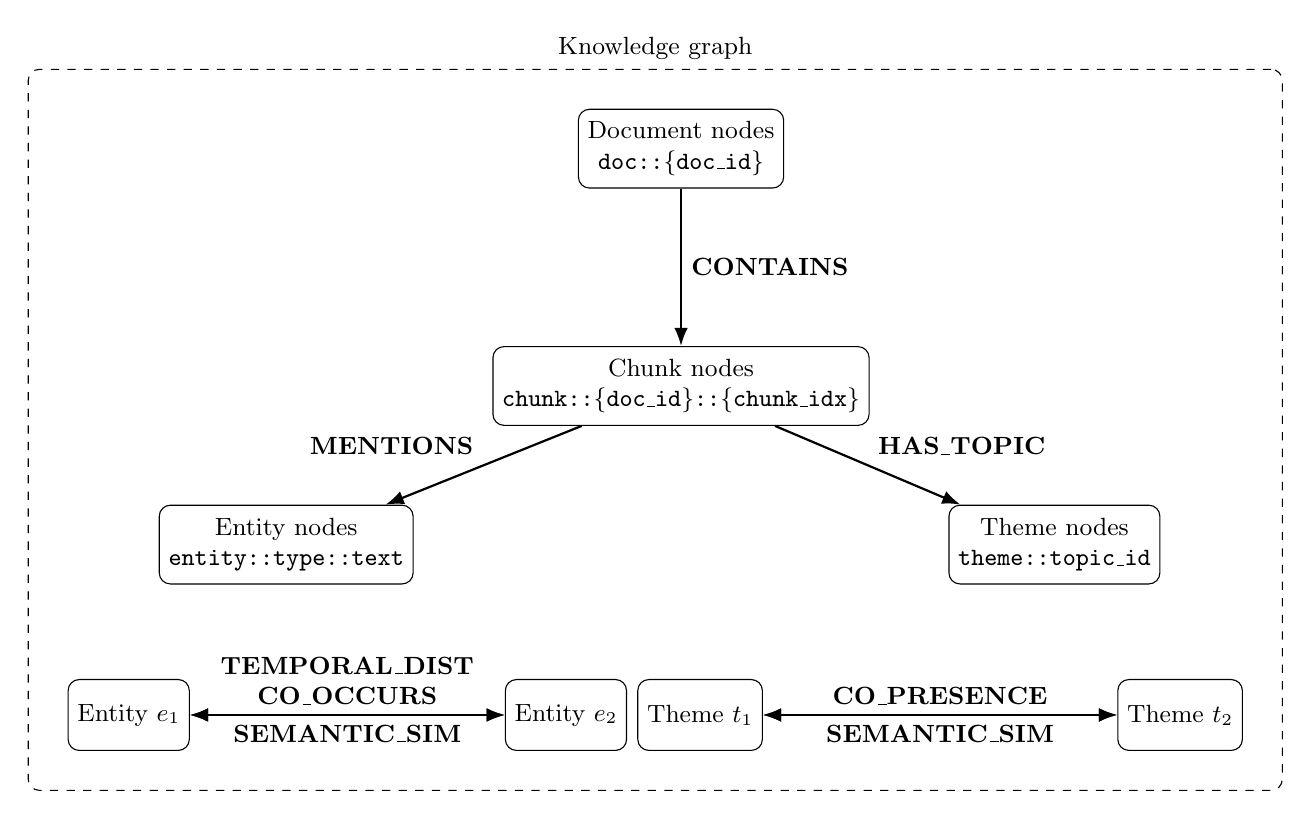
\begin{tikzpicture}[
        node distance=2cm,
        >=Latex,
        font=\small,
        block/.style={rectangle, draw, rounded corners, align=center, minimum width=1cm, minimum height=1cm},
        smallblock/.style={rectangle, draw, rounded corners, align=center, minimum width=0.5cm, minimum height=0.9cm},
        group/.style={rectangle, dashed, draw, rounded corners, inner sep=0.5cm},
        line/.style={->, thick}
    ]

    % Main node types (vertical)
    \node[block] (doc) {Document nodes\\\texttt{doc::\{doc\_id\}}};
    \node[block, below=of doc] (chunk) {Chunk nodes\\\texttt{chunk::\{doc\_id\}::\{chunk\_idx\}}};
    \node[block, below left=1cm and 1cm of chunk] (entity) {Entity nodes\\\texttt{entity::type::text}};
    \node[block, below right=1cm and 1cm of chunk] (theme) {Theme nodes\\\texttt{theme::topic\_id}};

    % Edges
    \draw[line] (doc) -- node[right, align=center] {\textbf{CONTAINS}} (chunk);
    \draw[line] (chunk) -- node[above left, align=center] {\textbf{MENTIONS}} (entity);
    \draw[line] (chunk) -- node[above right, align=center] {\textbf{HAS\_TOPIC}} (theme);

    % Entity--entity relationships
    \node[smallblock, below=1.2cm of entity, xshift=-2cm] (e1) {Entity $e_1$};
    \node[smallblock, right=4cm of e1] (e2) {Entity $e_2$};
    \draw[line, <->] (e1) -- node[above, align=center] {\textbf{TEMPORAL\_DIST} \\ \textbf{CO\_OCCURS}} (e2);
    \draw[line, <->] (e1) -- node[below, align=center] {\textbf{SEMANTIC\_SIM}} (e2);

    % Theme--theme relationships
    \node[smallblock, below=1.2cm of theme, xshift=-4.5cm] (t1) {Theme $t_1$};
    \node[smallblock, right=4.5cm of t1] (t2) {Theme $t_2$};
    \draw[line, <->] (t1) -- node[above, align=center] {\textbf{CO\_PRESENCE}} (t2);
    \draw[line, <->] (t1) -- node[below, align=center] {\textbf{SEMANTIC\_SIM}} (t2);

    \node[group, fit=(doc) (chunk) (entity) (theme) (e1) (e2) (t1) (t2),
          label=above:{Knowledge graph}] (graphbox) {};

    \end{tikzpicture}
    \caption{Graph overview. Documents are split into chunks; chunks are annotated with entities (spaCy NER) and themes (BERTopic). The graph links documents, chunks, entities, and themes through edges (CONTAINS, MENTIONS, HAS\_TOPIC, CO\_OCCURS, CO\_PRESENCE, SEMANTIC\_SIM, TEMPORAL\_DIST).}
    \label{fig:graph_overview}
\end{figure}

\subsection{Document and Chunk Nodes}

\paragraph{Document nodes.} Each fact-check article in the corpus is represented as a document node with a unique identifier. Document nodes are created directly from the CSV input, using the document's unique ID as the node identifier with format \texttt{doc::\{doc\_id\}}. Each document node stores the original metadata (\texttt{url}, \texttt{title}, \texttt{publisher\_name}, \texttt{publisher\_site}, \texttt{review\_date}) and serves as the root of a document-chunk hierarchy.

\paragraph{Sentence-based chunking with overlap.} To enable finer-grained retrieval while preserving local context, each document body is split into overlapping, sentence-aware chunks. The chunking algorithm operates as follows:

\begin{enumerate}[itemsep=2pt]
    \item \textbf{Sentence detection}: The document body is first segmented into individual sentences using a regex pattern that matches sentence-ending punctuation (period, exclamation mark, or question mark) followed by whitespace and a capital letter, or at the end of the text. This ensures sentences are split at natural boundaries.

    \item \textbf{Sentence accumulation}: Starting from the first sentence, sentences are accumulated into a current chunk until adding the next sentence would exceed the soft character limit (default: 500 characters). The soft limit ensures chunks never break mid-sentence---if a sentence would cause the chunk to exceed the limit, the current chunk is finalized and the sentence starts the next chunk.

    \item \textbf{Overlap computation}: After finalizing a chunk, the algorithm computes overlap by selecting sentences from the end of the previous chunk to include at the beginning of the next chunk. Sentences are selected in reverse order until the cumulative length of selected sentences reaches approximately the overlap threshold (default: 100 characters). This sentence-level overlap preserves semantic coherence across chunk boundaries.

    \item \textbf{Iteration}: Steps 2 and 3 repeat until all sentences are processed. The final chunk contains any remaining sentences.
\end{enumerate}

Each chunk is assigned a unique identifier with format \texttt{chunk::\{doc\_id\}::\{chunk\_idx\}}, where \texttt{chunk\_idx} is the zero-based index of the chunk within its parent document. Chunk nodes store the raw textual content, parent document ID, and chunk index.

\subsection{Theme Nodes}

Theme nodes represent automatically discovered topics in the corpus using BERTopic, a state-of-the-art topic modeling framework that combines transformer-based embeddings with clustering algorithms. The theme construction process involves topic discovery, keyword processing, and label generation.

\paragraph{Topic discovery with BERTopic.} Given the complete collection of chunk texts $\{c_1, c_2, \ldots, c_n\}$, we apply BERTopic to discover latent thematic structure. BERTopic operates in several stages: (1) it embeds each chunk text using a SentenceTransformer model (the same embedding model used for semantic retrieval, ensuring consistency), (2) it reduces dimensionality using UMAP (Uniform Manifold Approximation and Projection), (3) it clusters the reduced embeddings using HDBSCAN (Hierarchical Density-Based Spatial Clustering of Applications with Noise), and (4) it extracts representative keywords for each cluster using class-based TF-IDF.

The model is configured with \texttt{min\_topic\_size} $= 10$ (minimum cluster size) and \texttt{nr\_topics} $= \texttt{None}$ (automatic detection). This produces a topic assignment $t_i$ for each chunk $c_i$ and a topic probability distribution $P(t \mid c_i)$ indicating the confidence of the assignment. The outlier topic (topic ID $-1$) groups chunks that do not fit into any coherent cluster and is excluded from the graph.

\paragraph{Keyword processing.} BERTopic returns raw keywords for each topic ranked by relevance. To obtain cleaner and more informative topic representations, we apply a multi-step processing pipeline:

\begin{enumerate}[itemsep=2pt]
    \item \textbf{Initial extraction}: Extract the top 15 keywords with highest class-based TF-IDF scores
    \item \textbf{Stemming}: Apply an English Snowball stemmer (NLTK) to normalize morphological variants (e.g., ``election'' and ``elections'' share the same stem)
    \item \textbf{Score aggregation}: For keywords sharing the same stem, accumulate their TF-IDF scores
    \item \textbf{N-gram deduplication}: Remove redundant n-grams by checking if a multi-word keyword exists---if so, discard its component unigrams (e.g., if ``climate change'' is present, remove standalone ``climate'' and ``change'')
    \item \textbf{Truncation}: Select the top 10 deduplicated keywords by aggregated score
\end{enumerate}

This pipeline reduces redundancy and ensures keywords are maximally informative.

\paragraph{Label generation via LLM.} Each theme node requires a human-readable label. By default, labels are generated using a local LLM (Ollama serving LLaMA 3.1) via a structured prompt. The LLM receives the top 10 processed keywords and a sample of representative chunk texts from the topic, then generates a concise descriptive label (maximum 4 words). The prompt instructs the LLM to create a label that captures the essence of the topic without generic terms. If LLM generation is disabled (via build flag), labels are created by concatenating the top 3 keywords.

Each theme node is identified as \texttt{theme::\{topic\_id\}} and stores the topic ID, label, and processed keyword list. Theme nodes serve as semantic anchors in the graph, enabling thematic retrieval.

\subsection{Entity Nodes}

Entity nodes represent named entities (people, organizations, locations, dates, events, and demographic groups) extracted from chunk texts using spaCy's Named Entity Recognition (NER) system. The entity extraction process involves NER application, type filtering, normalization, and special handling for DATE entities.

\paragraph{Named entity extraction with spaCy.} For each chunk text, we apply spaCy's NER pipeline (model \texttt{en\_core\_web\_sm}), which identifies entity mentions and assigns them to predefined categories. SpaCy uses a multi-layer convolutional neural network trained on the OntoNotes 5 corpus, achieving high precision on entity recognition tasks.

We retain entities belonging to seven semantic types that are relevant for fact-checking:
\begin{itemize}[itemsep=2pt]
    \item \textbf{PERSON}: People, including fictional characters (e.g., ``Donald Trump,'' ``Bill Gates'')
    \item \textbf{ORG}: Organizations, companies, agencies, institutions (e.g., ``AFP,'' ``World Health Organization'')
    \item \textbf{GPE}: Geopolitical entities---countries, cities, states (e.g., ``France,'' ``New York,'' ``California'')
    \item \textbf{LOC}: Non-GPE locations such as mountain ranges, bodies of water (e.g., ``Pacific Ocean,'' ``Himalayas'')
    \item \textbf{DATE}: Absolute or relative dates or periods (e.g., ``2020,'' ``January 15, 2019,'' ``last year'')
    \item \textbf{EVENT}: Named events such as hurricanes, battles, wars, sports events (e.g., ``World War II,'' ``Hurricane Katrina'')
    \item \textbf{NORP}: Nationalities, religious groups, or political groups (e.g., ``American,'' ``Republican,'' ``Muslim'')
\end{itemize}

Entities of other types (e.g., MONEY, PERCENT, QUANTITY) are discarded as they provide limited retrieval value.

\paragraph{Normalization and filtering.} All entity text strings are lowercased to ensure consistent matching (e.g., ``trump'' and ``Trump'' map to the same entity node). Very short entities (length $\leq 2$ characters) are filtered out, as they are often extraction errors or uninformative tokens (e.g., single initials).

\paragraph{Special DATE entity handling.} DATE entities pose a unique challenge: spaCy recognizes many date formats (``January 15, 2020,'' ``last week,'' ``2019-08-30''), but preserving all variations would create excessive fragmentation. To address this, we apply a year-extraction filter: from any DATE mention, we extract a 4-digit year using the regex pattern \texttt{\textbackslash b(19|20)\textbackslash d\{2\}\textbackslash b}. For example, ``January 15, 2020'' $\rightarrow$ ``2020,'' and ``2019-08-30'' $\rightarrow$ ``2019.'' Relative dates without explicit years (e.g., ``last week'') are discarded. This reduces DATE node count while preserving meaningful temporal information for TEMPORAL\_DIST edges.

Each entity node is uniquely identified as \texttt{entity::\{entity\_type\}::\{entity\_text\}}, where \texttt{entity\_type} is one of the seven types and \texttt{entity\_text} is the normalized (lowercased) entity string. Entity nodes store the entity type and text, serving as connection points for entity-based retrieval.

\subsection{CONTAINS: Document $\to$ Chunk}

CONTAINS edges form the structural backbone of the graph, representing the hierarchical containment relationship between documents and their constituent chunks.

For each chunk node \texttt{chunk::\{doc\_id\}::\{chunk\_idx\}}, we create a directed edge from its parent document node \texttt{doc::\{doc\_id\}} to the chunk. The edge is assigned a uniform weight $w = 1.0$, as all chunks are equally part of their parent document. These edges enable upward traversal from retrieved chunks to their source documents during result aggregation.

\subsection{HAS\_TOPIC: Chunk $\to$ Theme}

HAS\_TOPIC edges connect chunks to theme nodes based on the topic probability distributions produced by BERTopic during theme discovery.

During BERTopic training (Section~\ref{sec:nodes}), each chunk $c$ is assigned a primary topic $t^*$ and a full probability distribution $P(t \mid c)$ over all topics. While the primary topic has the highest probability, chunks often have non-negligible probability mass on secondary topics, reflecting thematic overlap.

To capture both primary and secondary thematic associations, we create HAS\_TOPIC edges for all topic assignments above a confidence threshold $\tau_{\text{topic}}$ (default: $0.15$):
\[
\text{Create edge}(c, t) \quad \text{if} \quad P(t \mid c) > \tau_{\text{topic}}.
\]

The edge weight is set directly to the topic probability:
\[
w_{\text{HAS\_TOPIC}}(c, t) = P(t \mid c).
\]

This probabilistic weighting enables soft thematic assignment: chunks with strong confidence in a topic have high-weight edges, while chunks with ambiguous or mixed themes have multiple moderate-weight edges. During thematic retrieval, these weights modulate relevance propagation through the theme graph.

\subsection{MENTIONS: Chunk $\to$ Entity}

MENTIONS edges connect chunks to the entities they contain, weighted by a combination of term frequency (TF), inverse document frequency (IDF), and sigmoid normalization. This weighting scheme balances local salience (how prominently an entity appears in a chunk) with global discriminativeness (how rare the entity is across the corpus).

\paragraph{Local normalized TF-IDF computation.} For each entity $e$ mentioned in chunk $c$, we compute:

\begin{enumerate}[itemsep=2pt]
    \item \textbf{Term frequency (TF)}: Count how many times entity $e$ appears in chunk $c$, denoted $\text{TF}(e,c)$
    \item \textbf{Local normalization}: Normalize by the maximum TF of any entity in the chunk to obtain $\widetilde{\text{TF}}(e,c) = \frac{\text{TF}(e,c)}{\max_{e'} \text{TF}(e',c)}$. This ensures the most frequently mentioned entity in the chunk receives TF $= 1$, while less frequent entities receive fractional values
    \item \textbf{Inverse document frequency (IDF)}: Compute $\text{IDF}(e) = \log\left(\frac{N}{\text{df}(e)}\right)$, where $N$ is the total number of chunks and $\text{df}(e)$ is the document frequency (number of chunks containing $e$). Rare entities receive high IDF, common entities receive low IDF
    \item \textbf{TF-IDF product}: Combine as $w_{\text{raw}}(c,e) = \widetilde{\text{TF}}(e,c) \cdot \text{IDF}(e)$
\end{enumerate}

\paragraph{Sigmoid normalization.} Raw TF-IDF scores have unbounded range and heavy tails. To map them into $(0,1)$ and suppress extreme values, we apply a sigmoid function with scale parameter $s$ (default: $s=3.0$):
\[
w_{\text{MENTIONS}}(c,e) = \sigma\left(\frac{w_{\text{raw}}(c,e)}{s}\right) = \frac{1}{1 + \exp\left(-\frac{w_{\text{raw}}(c,e)}{s}\right)}.
\]

This produces smooth, bounded weights that emphasize salient and discriminative entity mentions while downweighting ubiquitous entities.

\subsection{CO\_OCCURS: Entity $\leftrightarrow$ Entity}

CO\_OCCURS edges capture entity co-occurrence patterns at the document level, connecting entities that frequently appear together in fact-check articles. These edges enable entity-based retrieval to expand from a query entity to related entities.

\paragraph{Special DATE entity handling.} DATE-DATE co-occurrences are \emph{excluded} from CO\_OCCURS edges because temporal relationships between years are captured by dedicated TEMPORAL\_DIST edges. However, DATE entities may co-occur with non-DATE entities (e.g., PERSON-DATE, ORG-DATE, GPE-DATE), which capture event-year associations valuable for retrieval.

\paragraph{Document-level co-occurrence counting.} We group chunks by their parent document and aggregate all entities mentioned in each document. For each pair of entities $(e_1, e_2)$ appearing in at least one common document, we count the number of documents containing both: $\text{count}(e_1, e_2)$. We also track the marginal document frequencies $\text{freq}(e_1)$ and $\text{freq}(e_2)$ (number of documents containing each entity individually).

\paragraph{PMI weighting with sigmoid.} Raw co-occurrence counts favor ubiquitous entities. To emphasize statistically significant associations, we compute Pointwise Mutual Information (PMI):
\[
\text{PMI}(e_1, e_2) = \log\left(\frac{\text{count}(e_1, e_2) \cdot N}{\text{freq}(e_1) \cdot \text{freq}(e_2)}\right),
\]
where $N$ is the total number of documents. PMI is positive when entities co-occur more frequently than expected under independence, and negative otherwise. We then apply sigmoid normalization (scale $s=2.0$) to map PMI into $(0,1)$:
\[
w_{\text{CO\_OCCURS}}(e_1, e_2) = \sigma\left(\frac{\text{PMI}(e_1, e_2)}{s}\right).
\]

Edges are created only when $\text{count}(e_1, e_2) \ge 2$ (minimum 2 co-occurrences) and at least one entity is non-DATE.

\subsection{CO\_PRESENCE: Theme $\leftrightarrow$ Theme}

CO\_PRESENCE edges connect themes that frequently co-appear in the same chunks, capturing thematic overlap and enabling multi-topic retrieval.

For each pair of themes $(t_1, t_2)$, we count the number of chunks where both themes exceed the HAS\_TOPIC threshold: $\text{count}(t_1, t_2)$. We normalize by the geometric mean of theme frequencies to penalize ubiquitous themes:
\[
w_{\text{CO\_PRESENCE}}(t_1, t_2) = \text{count}(t_1, t_2) \cdot \frac{1}{\sqrt{\text{freq}(t_1) \cdot \text{freq}(t_2)}}.
\]

This weighting balances raw co-presence counts with theme generality, ensuring edges reflect meaningful thematic associations.

\subsection{SEMANTIC\_SIM: Entity and Theme Similarity}

SEMANTIC\_SIM edges encode semantic similarity between entities or between themes, computed from embedding representations.

\paragraph{Entity semantic similarity.} For non-DATE entities, we compute cosine similarity between entity text embeddings. Entity texts (e.g., ``trump,'' ``world health organization'') are embedded using the same SentenceTransformer model used for chunks. For each pair of entities with cosine similarity above threshold $\tau_{\text{sem}}$ (default: $0.8$), we create an edge with weight equal to the similarity. DATE entities are excluded because temporal relationships are captured by TEMPORAL\_DIST.

\paragraph{Theme semantic similarity.} For themes, we concatenate the top 10 processed keywords into a single string, embed it, and compute pairwise cosine similarities. Edges are created for theme pairs exceeding $\tau_{\text{sem}} = 0.8$. This connects themes with similar keyword distributions, even if they do not frequently co-appear in chunks.

\subsection{TEMPORAL\_DIST: DATE $\leftrightarrow$ DATE}

TEMPORAL\_DIST edges connect DATE entity nodes (year nodes) based on temporal proximity, enabling retrieval to expand across related time periods.

For each pair of years $(y_1, y_2)$ within a maximum gap $\Delta_{\max}$ (default: $\Delta_{\max} = 10$ years), we compute an exponentially decaying similarity:
\[
w_{\text{TEMPORAL\_DIST}}(y_1, y_2) = \exp\left(-\lambda \, |y_1 - y_2|\right),
\]
with decay rate $\lambda = 0.15$. Adjacent years receive high weight ($\exp(-0.15) \approx 0.86$), while years 10 years apart receive weight $\exp(-1.5) \approx 0.22$. This allows retrieval to propagate temporally from a query year to nearby years, capturing evolving fact-check topics.

\subsection{Claim Nodes and REVIEWS Edges}

Claim nodes represent individual factual assertions that have been investigated and fact-checked, extracted directly from the dataset. Each claim is associated with structured metadata: a unique \texttt{claim\_id}, the claim \texttt{text} (the factual assertion), a \texttt{rating} (the verdict assigned by fact-checkers, e.g., ``False,'' ``Misleading,'' ``True''), the \texttt{claimant} (the person or entity who made the claim), and a \texttt{review\_date}. Claim nodes are identified as \texttt{claim::\{claim\_id\}}.

\paragraph{REVIEWS edges.} Each claim node is connected to its corresponding fact-checking document by a directed \textbf{REVIEWS} edge (claim $\to$ document). This edge encodes the semantic link between a factual assertion and the article that investigates it, enabling retrieval strategies to traverse from a query-similar claim directly to its associated fact-check document. These edges are the backbone of the three claim-based retrieval strategies (S5, S6, S7, described in Section~\ref{sec:retrieval}).

\paragraph{Pre-computed claim embeddings.} All claim texts are embedded offline using the same SentenceTransformer model as chunks. These embeddings are stored and indexed to allow efficient query-to-claim similarity computation at retrieval time without recomputing embeddings.

\section{Retrieval Strategies}
\label{sec:retrieval}

\subsection{Approach Overview}

Given a user query, the system retrieves relevant chunks using seven complementary strategies: (1) \textbf{Semantic Similarity} (S1, non-graph), direct embedding similarity between query and chunks; (2) \textbf{Topic Distribution Similarity} (S2, non-graph), Jensen-Shannon divergence between query and chunk topic distributions; (3) \textbf{Thematic Graph Traversal} (S3, graph-based), BFS traversal over theme nodes seeded by query topic distribution; (4) \textbf{Entity Graph Traversal} (S4, graph-based), BFS traversal over entity nodes seeded by query entities; (5) \textbf{Claim-Document Retrieval} (S5, claim-based), traversal from claims similar to the query to their associated documents via REVIEWS edges; (6) \textbf{Claim-Topic Distribution} (S6, claim-based), combining claim similarity with topic distribution alignment; and (7) \textbf{Claim-Keyphrase Similarity} (S7, claim-based), combining claim similarity with KeyBERT-extracted keyphrase matching.

Strategies S1--S2 provide direct similarity baselines; S3--S4 leverage graph structure for relevance propagation; S5--S7 exploit the claim layer to bridge between the query and previously verified factual assertions. All seven scores are fused by weighted average with weights $\alpha=0.50$ (S1), $\beta=0.03$ (S2), $\gamma=0.02$ (S3), $\delta=0.05$ (S4), $\varepsilon=0.15$ (S5), $\zeta=0.13$ (S6), $\eta=0.12$ (S7).

Figure~\ref{fig:retrieval_pipeline} shows the retrieval pipeline.

\begin{figure}[H]
    \centering
    \includegraphics[width=\textwidth]{retrieval_diagram.png}
    \caption{Retrieval pipeline: the user query is transformed into embeddings, topics, and entities. These feed four complementary retrieval strategies: semantic similarity (S1), topic distribution similarity (S2), thematic graph traversal (S3), and entity graph traversal (S4), which are then fused into a final score per chunk.}
    \label{fig:retrieval_pipeline}
\end{figure}

\subsection{Strategy 1: Semantic Similarity}

Semantic similarity is a non-graph baseline strategy that directly compares the query embedding to all chunk embeddings using cosine similarity.

\paragraph{Offline indexing.} During graph construction, all chunk texts are embedded using the SentenceTransformer model (all-MiniLM-L6-v2, 384 dimensions). These embeddings are stored in a FAISS index (Facebook AI Similarity Search), an efficient library for dense vector similarity search. FAISS uses approximate nearest neighbor algorithms (e.g., IVF with PQ compression) to enable sub-linear search over large embedding collections.

\paragraph{Online retrieval.} Given a query, we embed it using the same SentenceTransformer model, search the FAISS index for the top-$K$ most similar chunk embeddings by cosine similarity, and retrieve the corresponding chunks. Similarity scores are min-max normalized across the top-$K$ results to produce $\text{score}_{\text{sem}}(c) \in [0,1]$.

This strategy captures semantic similarity at the text level, retrieving chunks that paraphrase or discuss the same concepts as the query, even without keyword overlap.

\subsection{Strategy 2: Topic Distribution Similarity}

Topic distribution similarity is a non-graph baseline that compares the full topic distributions of the query and each chunk.

\paragraph{Jensen-Shannon divergence.} For each chunk $c$, we compute the Jensen-Shannon (JS) divergence between $P(t \mid \text{query})$ and $P(t \mid c)$:
\[
\text{JS}(P_{\text{query}}, P_c) = \frac{1}{2} \text{KL}(P_{\text{query}} \| M) + \frac{1}{2} \text{KL}(P_c \| M),
\]
where $M = \frac{1}{2}(P_{\text{query}} + P_c)$ and $\text{KL}$ is the Kullback-Leibler divergence. JS divergence is symmetric and bounded: $\text{JS} \in [0, \log 2]$.

\paragraph{Similarity conversion.} We convert divergence to similarity via $\text{score}_{\text{topic\_dist}}(c) = 1 - \frac{\text{JS}(P_{\text{query}}, P_c)}{\log 2}$, yielding scores in $[0,1]$.

This strategy captures coarse-grained thematic alignment based on topic distributions, complementing the finer-grained theme graph traversal.

\subsection{Strategy 3: Thematic Graph Traversal}

Thematic graph traversal is a graph-based strategy that leverages the theme layer to retrieve chunks via thematic associations.

\paragraph{Query topic inference.} We apply the trained BERTopic model to the query text to obtain a topic distribution $P(t \mid \text{query})$. This distribution assigns probabilities to each theme, indicating how strongly the query aligns with each topic.

\paragraph{Theme graph traversal via BFS.} We seed the theme graph with themes having $P(t \mid \text{query}) > \tau_{\text{theme}}$ (default: $0.1$), assigning initial relevance scores equal to the topic probabilities. We then propagate relevance through the theme graph using breadth-first search (BFS) over CO\_PRESENCE and theme SEMANTIC\_SIM edges, decaying relevance at each hop. Themes reached during BFS accumulate relevance from their incoming edges.

\paragraph{Chunk score accumulation.} After BFS completes, each theme node has a final relevance score. We traverse HAS\_TOPIC edges backwards from themes to chunks, accumulating chunk scores weighted by HAS\_TOPIC edge weights. Chunks connected to highly relevant themes receive high thematic scores. Scores are normalized to $[0,1]$.

This strategy retrieves chunks based on high-level thematic alignment, even if they do not share specific keywords or entities with the query.

\subsection{Strategy 4: Entity Graph Traversal}

Entity graph traversal leverages the entity layer to retrieve chunks via entity mentions and entity associations.

\paragraph{Query entity extraction.} We apply spaCy NER to the query text to extract entities, using the same types and normalization as during graph construction. Each extracted entity serves as a seed for graph traversal.

\paragraph{Entity graph traversal via BFS.} We seed the entity graph with query entities, assigning initial relevance $=1.0$. We then propagate relevance through CO\_OCCURS and entity SEMANTIC\_SIM edges via BFS, decaying at each hop and filtering by edge weight and relevance thresholds. Entities reached during BFS accumulate relevance.

\paragraph{Chunk score accumulation.} After BFS, we traverse MENTIONS edges backwards from entities to chunks, accumulating chunk scores weighted by MENTIONS edge weights. Chunks mentioning highly relevant entities receive high entity scores. Scores are normalized to $[0,1]$.

This strategy expands from query entities to related entities (e.g., from ``Trump'' to ``Republican Party'' or ``2016''), then retrieves chunks mentioning those entities.

\subsection{Strategies S5--S7: Claim-Based Retrieval}

Strategies S5, S6, and S7 exploit the claim layer of the knowledge graph. All three share a common first step: embedding the query and computing cosine similarity to all pre-indexed claim embeddings to find the top-$k$ most similar claims (default $k=10$). Claims above a threshold are also expanded by claim-to-claim embedding similarity (effective similarity: $\text{query\_sim}(c_i) \times \cos(c_i, c_j)$) to reach semantically related but not directly matched claims.

\paragraph{S5: Claim-Document Retrieval.} For each matched claim, we traverse REVIEWS edges to its associated document, then CONTAINS edges to retrieve all chunks of that document. Each chunk receives a score equal to the maximum cosine similarity between the query and any matched claim reaching that document:
\[
S_5(c) = \max_{\text{matched claims}} \cos(\text{embed}(\text{query}),\, \text{embed}(\text{claim})).
\]

\paragraph{S6: Claim-Topic Distribution.} This strategy combines claim matching with topic distribution alignment. For each chunk reached via REVIEWS, the score is a product of three factors:
\[
S_6(c) = \text{claim\_sim} \times \text{topic\_sim} \times \text{topic\_confidence},
\]
where $\text{topic\_sim} = 1 - \text{JSD}(P_{\text{query}}, P_c)$ and $\text{topic\_confidence}$ is the maximum HAS\_TOPIC weight for the chunk's topics (default $0.5$ if no topic is assigned). All factors are in $[0,1]$, so $S_6 \in [0,1]$.

\paragraph{S7: Claim-Keyphrase Similarity.} This strategy combines claim matching with keyphrase-level evidence. The query is first processed by KeyBERT to extract the top-$n$ most salient keyphrases (default $n=5$). For each chunk reached via REVIEWS, we compute cosine similarity between each extracted keyphrase embedding and the chunk embedding, and score:
\[
S_7(c) = \text{claim\_sim} \times \text{keyphrase\_sim} \times \text{keyphrase\_importance},
\]
where $\text{keyphrase\_sim}$ is the maximum cosine similarity between any query keyphrase and the chunk, and $\text{keyphrase\_importance}$ is the KeyBERT relevance score for the best-matching keyphrase.

\subsection{Score Fusion}

Each strategy produces a normalized score per chunk in $[0,1]$. We combine all seven scores via weighted average:
\[
\text{score}_{\text{final}}(c) = \alpha \, S_1(c) + \beta \, S_2(c) + \gamma \, S_3(c) + \delta \, S_4(c) + \varepsilon \, S_5(c) + \zeta \, S_6(c) + \eta \, S_7(c),
\]
where $\alpha + \beta + \gamma + \delta + \varepsilon + \zeta + \eta = 1$. Default weights are $\alpha=0.50$, $\beta=0.03$, $\gamma=0.02$, $\delta=0.05$, $\varepsilon=0.15$, $\zeta=0.13$, $\eta=0.12$, placing the strongest emphasis on direct semantic similarity while giving significant combined weight to the three claim-based strategies ($\varepsilon + \zeta + \eta = 0.40$).

Chunks from all strategies are aggregated, sorted by $\text{score}_{\text{final}}(c)$ in descending order, and the top-$K$ are returned. Document-level scores are then computed via softmax pooling over chunks within each document (sharpness parameter $\beta_{\text{soft}}=5.0$), enabling document-level ranking from chunk-level evidence.

\section{Evaluation}
\label{sec:results}

\subsection{Knowledge Graph Statistics}

The knowledge graph constructed from the first 5,000 documents of the corpus results in the node and edge counts shown in Table~\ref{tab:kg_stats}.

\begin{table}[H]
\centering
\begin{tabular}{lr}
\toprule
\textbf{Node Type} & \textbf{Count} \\
\midrule
Document & 5,000 \\
Chunk & $\sim$41,000 \\
Theme & $\sim$300 \\
Entity & $\sim$40,000 \\
Claim & $\sim$5,000 \\
\midrule
\textbf{Total Nodes} & $\sim$91,300 \\
\bottomrule
\end{tabular}
\quad
\begin{tabular}{lr}
\toprule
\textbf{Edge Type} & \textbf{Count} \\
\midrule
CONTAINS & $\sim$41,000 \\
MENTIONS & $\sim$177,000 \\
HAS\_TOPIC & $\sim$35,000 \\
CO\_PRESENCE & $\sim$315 \\
SEMANTIC\_SIM\_THEME & $\sim$9 \\
CO\_OCCURS & $\sim$100,000 \\
SEMANTIC\_SIM\_ENTITY & $\sim$30,000 \\
TEMPORAL\_DIST & $\sim$680 \\
REVIEWS & $\sim$5,000 \\
\midrule
\textbf{Total Edges} & $\sim$389,000 \\
\bottomrule
\end{tabular}
\caption{Knowledge graph statistics (5,000 documents; approximate counts).}
\label{tab:kg_stats}
\end{table}

\subsection{Benchmark Construction}

\paragraph{Dataset.} The benchmark is derived from a collection of social media posts (tweets), each associated with a ground-truth fact-checking document that verifies or refutes the claim made in the post. The ground-truth link is provided in a \texttt{relations.csv} file mapping each tweet identifier to the corresponding document identifier in the corpus.

A representative example is the following tweet:

\begin{quote}
\small
\textit{``Exclusive Footage from Kashmir Highway, Islamabad. Huge crowd came from KP, according to the ground reports.''}
\end{quote}

whose ground-truth fact-check document (doc\_id=1756) is titled:

\begin{quote}
\small
\textit{``Video shows traffic jam in Los Angeles, not roads near Imran Khan rally in Pakistan.''}
\end{quote}

\paragraph{Query reformatting.} Raw tweets are often noisy: they contain URLs, hashtags, \texttt{@}-mentions, emojis, and social-media jargon that degrade retrieval quality. We preprocess each tweet into a clean factual claim using LLaMA~3.1 (served locally via Ollama), with a structured prompt instructing the model to extract the core assertion, remove all noise, and rephrase as a concise 1--2 sentence factual statement. For example:

\begin{quote}
\small
\textbf{Tweet:} \textit{``..man, what time is the Trump arrest? Shit. https://t.co/xxx''}\\
\textbf{Reformatted:} \textit{Donald Trump was arrested on criminal charges.}
\end{quote}

\paragraph{Evaluation protocol.} We evaluate on 500 queries sampled from the benchmark. For each query, we run the full hybrid pipeline and record whether the ground-truth document appears in the top-$K$ retrieved documents (Hit@$K$ for $K \in \{1, 5, 10\}$), and compute the Mean Reciprocal Rank (MRR). We compare against the S1 semantic-only baseline (plain embedding cosine similarity, equivalent to classical RAG).

\subsection{Quantitative Results}

Table~\ref{tab:results} reports Hit@$K$ and MRR for both the full pipeline and the S1 semantic baseline.

\begin{table}[H]
\centering
\begin{tabular}{lcccc}
\toprule
\textbf{System} & \textbf{Hit@1} & \textbf{Hit@5} & \textbf{Hit@10} & \textbf{MRR} \\
\midrule
S1 Semantic (classic RAG) & 11\% & 60\% & 80\% & -- \\
Full Pipeline (7 strategies) & \textbf{47\%} & \textbf{70\%} & 80\% & -- \\
\bottomrule
\end{tabular}
\caption{Retrieval performance on 500 benchmark queries. Hit@$K$ = fraction of queries where the ground-truth document appears in the top-$K$ results.}
\label{tab:results}
\end{table}

\paragraph{Observations.} The full pipeline substantially outperforms the semantic baseline at low ranks: Hit@1 improves from 11\% to 47\% (+36 pp), and Hit@5 from 60\% to 70\% (+10 pp). Both systems converge at Hit@10=80\%, suggesting the graph-based signals primarily help the system \emph{rank relevant documents higher} rather than recovering entirely new documents. This is consistent with the role of claim-based strategies (S5--S7): they provide direct bridges from the query to relevant documents via previously verified claims, bypassing the need for high semantic similarity at the chunk level.

\subsection{Case Study: Qualitative Analysis on the Trump/Egypt/Ethiopia Query}

We also performed a qualitative inspection on a specific query to understand which signals drive retrieval. For the query \emph{``Donald Trump tweet that Egypt might `blow up' Ethiopia's dam''}, the top retrieved chunks include highly relevant content (e.g., chunks explicitly mentioning Trump's remark and Egypt's reaction) alongside false positives driven by high entity scores for ``Trump'' connected to unrelated political stories. This confirms that entity graph traversal can over-amplify hub nodes, and that the claim-based strategies add complementary precision by routing through verified factual assertions rather than raw entity co-occurrence.

\subsection{Adversarial Cases: Graph-RAG Recovers What Semantic Search Misses}

A key qualitative finding from our evaluation is the identification of cases where the hybrid pipeline retrieves a highly relevant document that pure semantic search ranks far too low. We define an \emph{adversarial case} as one where the top-1 document returned by the full pipeline does not appear in the top-10 results of the S1 semantic baseline.

\paragraph{Example.} Consider the query:

\begin{quote}
\small
\textit{A toxic chemicals train blast occurred in Ohio.}
\end{quote}

The hybrid pipeline ranks at position 1 the document:

\begin{quote}
\small
\textit{``After a derailed train in February 2023 sparked a massive fire and the release of toxic chemicals in a small Ohio village...''}
\end{quote}

This document is directly relevant to the query yet appears only at rank 13 in the S1 semantic baseline. The graph-based retrieval recovers it via claim and entity signals (shared entities: Ohio, toxic chemicals, train; claim similarity to pre-verified assertions about the incident) that are not captured by direct chunk-level embedding similarity.

\paragraph{Adversarial benchmark construction.} Running our pipeline on 500 benchmark queries, we identified \textbf{22 candidate adversarial cases} where the pipeline's top-1 document was absent from the S1 top-10. Manual inspection of these 22 cases revealed:

\begin{itemize}[itemsep=2pt]
    \item \textbf{$\sim$5 confirmed adversarial examples}: queries where the pipeline top-1 document is genuinely relevant and meaningfully better ranked than by S1 (e.g., the Ohio train blast, misinformation about protest crowd videos, fabricated arrest imagery).
    \item \textbf{Remaining cases}: queries that are too vague or ambiguous to draw a clear conclusion---the tweet provides insufficient factual content to determine whether the pipeline's top-1 document is the correct one (e.g., tweets consisting primarily of hashtags, @-mentions, or single-sentence reactions without a clear claim).
\end{itemize}

This analysis suggests that a subset of social media posts constitutes a natural adversarial benchmark for fact-check retrieval: cases where surface-level semantic similarity is misleading, and deeper structural signals (entity co-occurrence, claim matching, topic distribution) are required to surface the correct document. Constructing and curating such a benchmark---filtering out ambiguous queries and verifying relevance judgments---is a promising direction for future work.


\section{Conclusion}
\label{sec:conclusion}

We presented a knowledge graph-based retrieval system for fact-checking that represents 5,000 English fact-check articles as a multi-level graph with five node types (documents, chunks, themes, entities, claims) and eight edge types (CONTAINS, HAS\_TOPIC, MENTIONS, CO\_OCCURS, CO\_PRESENCE, SEMANTIC\_SIM, TEMPORAL\_DIST, REVIEWS). The graph explicitly encodes structural hierarchy, thematic associations, entity mentions, co-occurrence patterns, semantic similarity, temporal proximity, and links between verified claims and their source documents.

Our hybrid retrieval strategy combines seven complementary approaches fused by weighted average. Quantitative evaluation on 500 benchmark queries shows that the full pipeline achieves Hit@1=47\%, Hit@5=70\%, and Hit@10=80\%, versus 11\%, 60\%, and 80\% for a semantic-only baseline. The graph-based system substantially improves precision at low ranks (Hit@1 +36 pp, Hit@5 +10 pp), while both systems converge at Hit@10---confirming that the graph-based signals primarily help rank relevant documents higher rather than recovering entirely new ones.

Key takeaways from our work:

\begin{itemize}[itemsep=2pt]
    \item \textbf{Claim-based strategies are the dominant improvement}: The three claim-based retrieval strategies (S5--S7, combined weight 0.40) provide direct bridges from the query to relevant documents via previously verified factual assertions, bypassing the need for high chunk-level semantic similarity
    \item \textbf{Graph representation enables multi-hop retrieval}: Entity and theme traversal expand beyond direct keyword matches by propagating relevance through structural associations
    \item \textbf{Entity co-occurrence is a double-edged sword}: Entity expansion improves recall but risks over-amplifying hub nodes (e.g., ``Trump''); regularization remains an open challenge
    \item \textbf{Adversarial cases expose the limits of semantic search}: Our pipeline identifies cases where structural signals (entity co-occurrence, claim matching, topic distribution) recover relevant documents that pure embedding similarity ranks outside the top 10
\end{itemize}

\paragraph{Adversarial benchmark.} A secondary contribution of this work is the identification of a methodology for constructing an adversarial evaluation benchmark. By collecting cases where the pipeline's top-1 document is absent from the semantic baseline's top-10, we obtain a set of candidates that are hard for classical RAG but potentially recoverable by graph-based methods. Out of 500 queries, 22 such candidates were identified, of which approximately 5 were confirmed through manual inspection as genuine cases where the graph-based retrieval is superior. The remaining cases corresponded to queries too vague or noisy to allow confident relevance judgments, highlighting the need for query quality filtering in benchmark construction.

\paragraph{Future work.} To further improve the system, we plan to: (1) regularize entity graph traversal to reduce false positives by down-weighting hub nodes and limiting propagation depth, (2) enrich the theme layer with finer-grained topics and denser theme-to-theme connectivity, (3) optimize fusion weights via cross-validation on the labeled benchmark, (4) curate and expand the adversarial benchmark by filtering ambiguous queries, and (5) explore alternative relevance propagation methods (e.g., personalized PageRank) to replace BFS traversal.

While this work focuses on fact-checking, the approach generalizes to other domains requiring claim-based retrieval over large corpora with recurring entities and themes, such as legal case law, scientific literature, or policy documents.

\begin{thebibliography}{9}

\bibitem{manolescuRDFintro}
Ioana Manolescu.
\newblock \emph{Graph data format for the Web: RDF} (course slides / lecture material).
\newblock Big Graph Databases (ECE\_5DA04\_TP).

\bibitem{balalau2024factcheckbureau}
Oana Denisa Balalau, Pablo Bertaud-Velten, Younes El-Fraihi, Garima Gaur, Oana Goga, Samuel S. Guimar{\~a}es, Ioana Manolescu, and Brahim Saadi.
\newblock FactCheckBureau: Build Your Own Fact-Check Analysis Pipeline.
\newblock \emph{Proceedings of CIKM 2024}, 2024.

\bibitem{zhang2025graphrag}
Zhang et al.
\newblock GraphRAG: Graph-Based Retrieval-Augmented Generation.
\newblock \emph{arXiv:2503.04338}, 2025.

\bibitem{msftgraphrag}
Microsoft.
\newblock GraphRAG pipeline and tooling (technical documentation / open-source project).

\end{thebibliography}

\newpage
\onecolumn
\appendix

\section{Example Fact-Check Article}
\label{app:example}

This appendix presents a complete example of a fact-check article from our dataset, as provided by the Inria Saclay research lab.

\subsection{Article Metadata}

\begin{itemize}[itemsep=3pt]
    \item \textbf{ID}: 0
    \item \textbf{URL}: \url{https://factcheck.afp.com/11-year-old-photo-gaza-not-recent-violence-indian-kashmir}
    \item \textbf{Publisher}: AFP Fact Check (\texttt{factcheck.afp.com})
    \item \textbf{Review Date}: 2019-08-30
    \item \textbf{Language}: English
\end{itemize}

\subsection{Article Title}

\textit{``This is an 11-year-old photo from Gaza, not from recent violence in Indian Kashmir''}

\subsection{Article Body (excerpt)}

\begin{quote}
\small
A photo of a wounded woman and child has been shared multiple times on Facebook and Twitter alongside a claim it was taken in Indian Kashmir. The claim is false; the photo is from 2008 and was taken after an Israeli attack on a refugee camp in Gaza.

The photo was shared in a Facebook post here on August 22, 2019, and has since been shared more than 900 times.

A caption alongside the photo says: ``Faces tell the story!! India's brutality has turned Kashmir into a living hell...''

The photo has also been shared in several other Facebook posts, for example here, here, here and here, and on Twitter here, here, here and here, with a similar claim.

The same photo was also shared in multiple Facebook posts with a similar claim in 2013, for example here and here.

The photo of the wounded woman and boy was actually taken by Getty Images' photographer Adib Katib after an Israeli missile struck a refugee camp in Gaza on December 29, 2008.

A reverse image search on Google found the photo was published here in a report on the website of the Belfast Telegraph, an Irish daily, on December 29, 2008.

The report's headline reads: ``Israel declares 'war to the bitter end'.''

The photo caption reads: ``Samera Baalusha (34) carries her surviving child Mohamad (15 months) while she waits to see the body of her daughter Jawaher Baalusha [...]''
\end{quote}

\subsection{Key Characteristics}

This example illustrates typical features of fact-check articles in our corpus:

\begin{enumerate}[itemsep=3pt]
    \item \textbf{Clear verdict}: The article explicitly states ``The claim is false''
    \item \textbf{Evidence-based analysis}: Provides verifiable sources (Getty Images, Belfast Telegraph)
    \item \textbf{Context}: Explains the true origin of the photo (Gaza, 2008) and the false claim (Kashmir, 2019)
    \item \textbf{Named entities}: References to locations (Gaza, Kashmir, India, Israel), people (Samera Baalusha, Mohamad, Adib Katib), organizations (Getty Images, Belfast Telegraph), and dates (2008, 2013, 2019-08-22)
    \item \textbf{Recurring themes}: Misinformation about geopolitical conflicts, photo manipulation, viral social media claims
    \item \textbf{Cross-references}: Links to multiple social media posts spreading the same false claim
\end{enumerate}

\subsection{Relevance for Knowledge Graph Construction}

This article would be processed by our system as follows:

\begin{itemize}[itemsep=3pt]
    \item \textbf{Document node}: Created with ID 0
    \item \textbf{Chunk nodes}: Body segmented into $\sim$6--8 sentence-based chunks with 100-character overlap
    \item \textbf{Entity nodes}: Extracted entities include GPE (Gaza, Kashmir, India, Israel), PERSON (Samera Baalusha, Mohamad, Adib Katib), ORG (AFP, Getty Images, Belfast Telegraph, Facebook, Twitter), DATE (2008, 2013, 2019)
    \item \textbf{Theme nodes}: Likely topics include ``geopolitical conflicts,'' ``photo verification,'' ``social media misinformation''
    \item \textbf{Edges}: MENTIONS edges link chunks to entities; CO\_OCCURS edges connect frequently co-occurring entities (e.g., Gaza--Israel, Kashmir--India); TEMPORAL\_DIST edges link years (2008--2013--2019)
\end{itemize}

Given a user query such as ``Photo shows violence in Kashmir,'' our retrieval system would:
\begin{enumerate}[itemsep=3pt]
    \item Identify entities (Kashmir) and themes (violence, geopolitical conflict)
    \item Retrieve semantically similar chunks via embedding similarity
    \item Traverse entity graph to find related contexts (Gaza, Israel, photo verification)
    \item Rank this article highly due to direct entity matches and thematic relevance
\end{enumerate}

\end{document}
